\documentclass[
	12pt, % Default font size, values between 10pt-12pt are allowed
	%letterpaper, % Uncomment for US letter paper size
	%spanish, % Uncomment for Spanish
]{fphw}

% Template-specific packages
\usepackage[utf8]{inputenc} % Required for inputting international characters
\usepackage[T1]{fontenc} % Output font encoding for international characters
\usepackage{mathpazo} % Use the Palatino font
\usepackage{booktabs} % Required for better horizontal rules in tables
\usepackage{enumerate} % To modify the enumerate environment

\usepackage{amsmath}
\usepackage{amssymb}
\usepackage{enumitem}
\usepackage{graphicx}
\usepackage{xcolor}
\definecolor{hlink}{HTML}{000099}
\usepackage[colorlinks=true, allcolors=hlink]{hyperref}
\usepackage[square,numbers]{natbib}
\usepackage{float}
\usepackage[title]{appendix}
\usepackage{tabularx}
\usepackage{multirow}
\usepackage{multicol}
\usepackage{longtable}
\usepackage{listings}

\usepackage{textcomp}
\usepackage{listings}
\usepackage{xcolor}
\usepackage{filecontents}

\usepackage{pgfplots}
\usepackage{pgfplotstable}
\pgfplotsset{compat=1.9}

\geometry{top=1in}

\setlength{\parindent}{0pt}
\setlength{\parskip}{10pt}

\bibliographystyle{unsrt}

\newcommand{\refeq}[1]{\hyperref[#1]{(\ref*{#1})}}
\newcommand{\refseq}[1]{\hyperref[#1]{section \ref*{#1}}}
\newcommand{\reftab}[1]{\hyperref[#1]{table \ref*{#1}}}
\newcommand{\reffig}[1]{\hyperref[#1]{figure \ref*{#1}}}
\newcommand{\reflst}[1]{\hyperref[#1]{listing \ref*{#1}}}
\newcommand{\refcode}[1]{\hyperref[#1]{(Code to test it)}}
\newcommand{\note}[1]{\textbf{\textcolor{blue}{{NOTE: #1}}}}

\title{Rocket League}
\author{Pasquale De Marinis}

\institute{University of Bari \\ Department of Computer Science} % Institute or school name
\class{Big Data} % Course or class name
\professor{Michelangelo Ceci} % Professor or teacher in charge of the assignment

\begin{document}

\maketitle
\tableofcontents\newpage

\section{Introduction}

This case study deals with the practical application of the Cross Industry Standard Process for Data Mining, in short CRISP-DM. The main objective is the analysis of Rocket League match replays in order to predict the skill of each player in a specific match.

This documentation will follow the six phases of CRISP-DM, thus in each section, a phase will be described, however the process is iterative, therefore it will anticipate in each section analysis that can be chronologically distant.
\section{Business understanding} \label{seq:business}

 In this phase the objective is to determine and understand the context and the scope of the project. So it has a lot in common with the initial steps of any significant project undertaking.

\begin{figure}[h]
    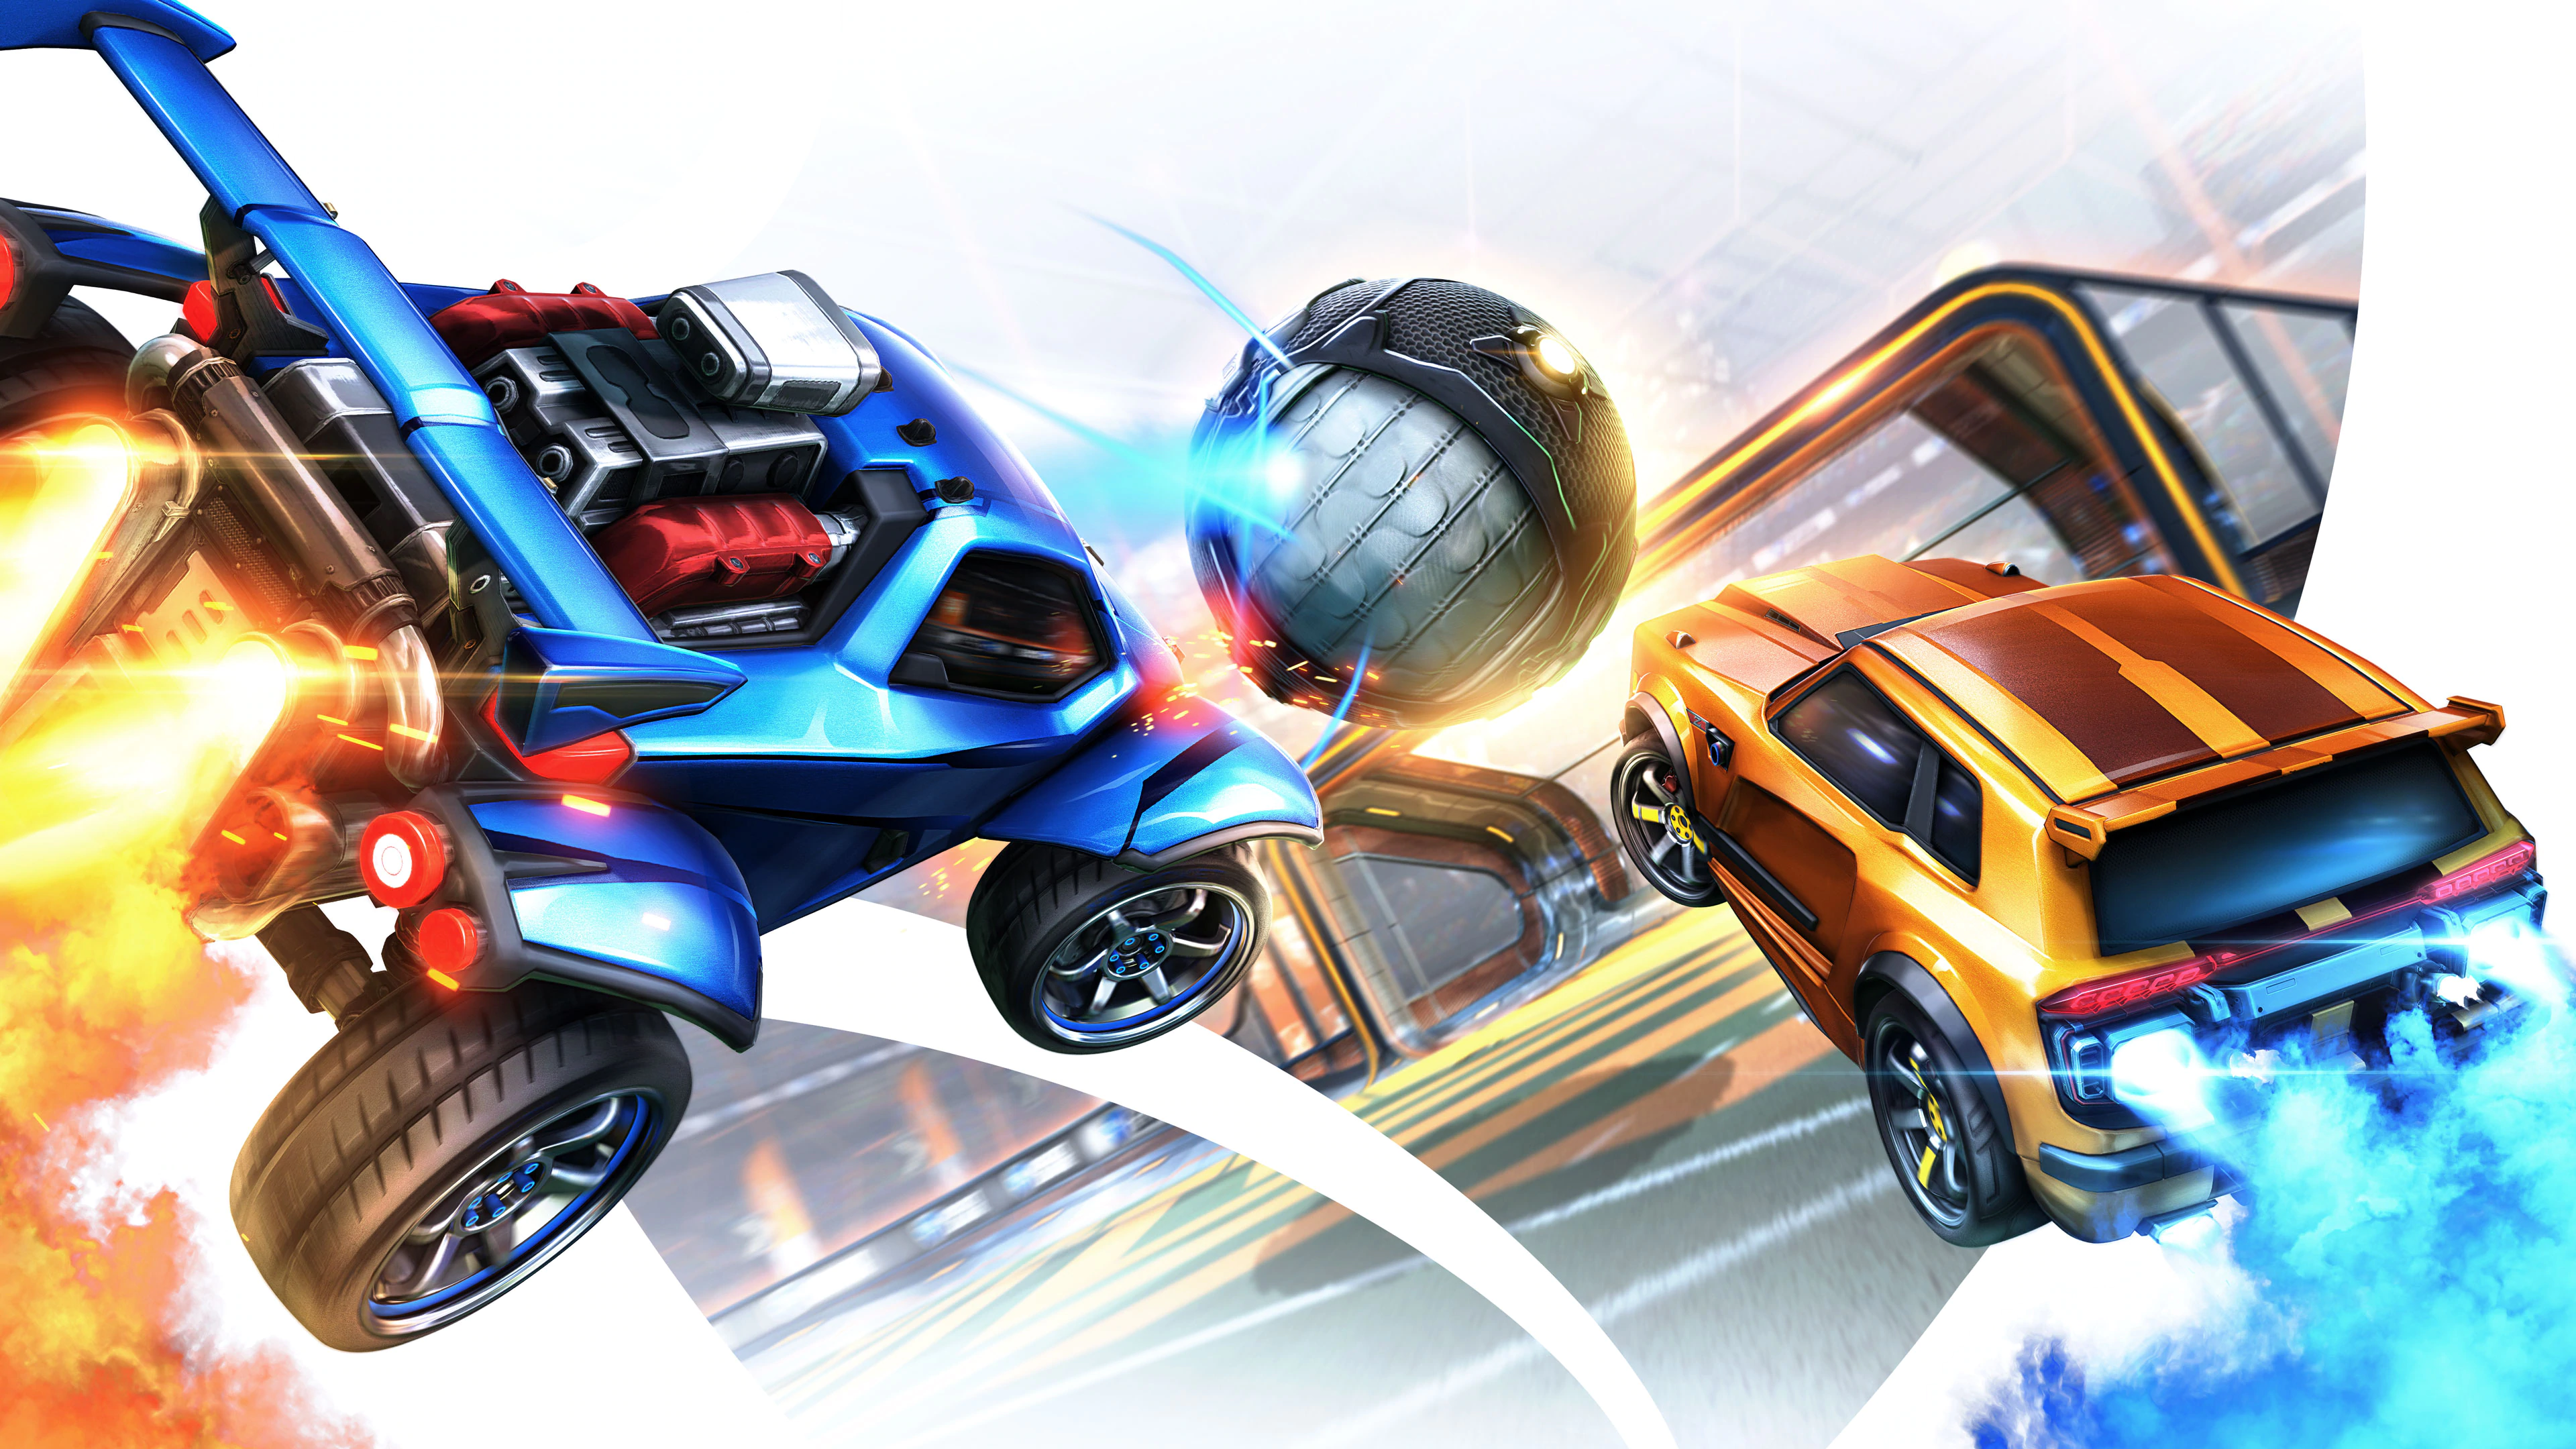
\includegraphics[width=\linewidth]{res/RL}
    \caption{One of the main Rocket League artworks}
\end{figure}

In recent years video games gained a lot of popularity, above all, multiplayer games; some of this are considered competitive and many sportive events take place around them.
Rocket League is a multiplayer competitive online game which is an hybrid that unifies soccer with car race games.

Thus, each match follows more or less soccer rules, but instead of human players there are cars controlled by the players. The number of players per team can be 1 (duel), 2, or 3 (standard). In our study we will focus on the main modality, that is 3vs3.

\subsubsection{Ranking System}

\begin{figure}[h]
    \includegraphics[width=\linewidth]{res/rankings}
    \caption{Rocket league rankings}
    \label{fig:ranks}
\end{figure}

In each modality, the player, after playing 10 competitive- online matches, is classified into a rank, based on the result of the 10 played matches. The ranks (visually shown in \reffig{fig:ranks}) are: 


\begin{multicols}{3}
    \begin{itemize}
        \item Bronze I
        \item Silver I
        \item Gold I
        \item Platinum I      
        \item Diamond I        
        \item Champion I         
        \item Grand Champion I    
        \item Bronze II
        \item Silver II
        \item Gold II       
        \item Platinum II     
        \item Diamond  II         
        \item Champion II         
        \item Grand Champion II
        \item Bronze III
        \item Silver III
        \item Gold III    
        \item Platinum III     
        \item Diamond  III        
        \item Champion III         
        \item Grand Champion III
    \end{itemize}
\end{multicols}

\begin{itemize}
    \item Supersonic Legend
\end{itemize}

Each rank, is split in four divisions (Division I, II, III and IV). And, each rank with its divisions is itself a discretization of a number, that is the Match Making Ranking (MMR). 
The MMR goes from 0 to potentially infinity, however the last rank: Supersonic Legend, takes the interval [1861, +Infinity]. A detailed view on MMRs and rankings is shown in \reftab{tab:mmrs}.

When the player starts playing, it is assigned an MMR of 600, that correspond to Gold III Division II. The MMR increase or decrease basing on the outcome of the matches it plays, obviously if he wins it will increase, viceversa if he loses. How much it can gain or lose at the end of the match is based on the number of played matches. In the first match, the gain/loss is +/-150. In the second match the values is halved, and after, it logarithmically decrease, until after some dozen of matches, it converge to +/- 10.

With this system, the player, will be classified in its most appropriate rank after a few dozen of matches and, therefore will compete with players of the same skill level.
Ranking, is also only determined by the outcome of the match, making the player experience frustrating in some cases. These are the business problems, thus the opportunity is making a more fast ranking system, and also more fair, taking in account the performance of the player in the match, in order to give also a meritocratic system.

\subsection{Determine Business Objectives}

Our business objective is, therefore:
\begin{itemize}
    \item Predict the rank of a player from the skill shown during the match
\end{itemize}
\begin{table}[]
    \begin{tabular}{|l|c|c|c|c|}
    \hline
    \textbf{Tier}                 & \multicolumn{1}{l|}{\textbf{Division I}} & \multicolumn{1}{l|}{\textbf{Division II}} & \multicolumn{1}{l|}{\textbf{Division III}} & \multicolumn{1}{l|}{\textbf{Division IV}} \\ \hline
    \textbf{Supersonic   Legend}  & 1.861 — 2.008                            & —                                         & —                                          & —                                         \\ \hline
    \textbf{Grand Champion   III} & 1.709 — 1.739                            & 1.745 — 1.773                             & 1.788 — 1.814                              & 1.832 — 1.860                             \\ \hline
    \textbf{Grand Champion   II}  & 1.575 — 1.598                            & 1.600 — 1.636                             & 1.638 — 1.660                              & 1.677 — 1.701                             \\ \hline
    \textbf{Grand Champion I}     & 1.435 — 1.458                            & 1.460 — 1.494                             & 1.498 — 1.527                              & 1.537 — 1.559                             \\ \hline
    \textbf{Champion III}         & 1.315 — 1.333                            & 1.335 — 1.366                             & 1.368 — 1.394                              & 1.402 — 1.420                             \\ \hline
    \textbf{Champion II}          & 1.195 — 1.213                            & 1.215 — 1.246                             & 1.248 — 1.275                              & 1.282 — 1.300                             \\ \hline
    \textbf{Champion I}           & 1.075 — 1.093                            & 1.095 — 1.127                             & 1.128 — 1.148                              & 1.162 — 1.180                             \\ \hline
    \textbf{Diamond III}          & 995 — 1.003                              & 1.004 — 1.027                             & 1.028 — 1.051                              & 1.052 — 1.060                             \\ \hline
    \textbf{Diamond II}           & 915 — 923                                & 924 — 947                                 & 948 — 971                                  & 972 — 980                                 \\ \hline
    \textbf{Diamond I}            & 835 — 843                                & 844 — 867                                 & 868 — 891                                  & 892 — 900                                 \\ \hline
    \textbf{Platinum III}         & 773 — 778                                & 779 — 797                                 & 798 — 816                                  & 817 — 825                                 \\ \hline
    \textbf{Platinum II}          & 715 — 718                                & 719 — 737                                 & 738 — 756                                  & 757 — 765                                 \\ \hline
    \textbf{Platinum I}           & 655 — 658                                & 659 — 677                                 & 678 — 696                                  & 697 — 705                                 \\ \hline
    \textbf{Gold III}             & 595 — 598                                & 599 — 617                                 & 618 — 636                                  & 637 — 643                                 \\ \hline
    \textbf{Gold II}              & 535 — 538                                & 539 — 557                                 & 558 — 576                                  & 577 — 585                                 \\ \hline
    \textbf{Gold I}               & 475 — 478                                & 479 — 497                                 & 498 — 516                                  & 517 — 524                                 \\ \hline
    \textbf{Silver III}           & 415 — 418                                & 419 — 437                                 & 438 — 456                                  & 457 — 467                                 \\ \hline
    \textbf{Silver II}            & 355 — 358                                & 359 — 377                                 & 378 — 396                                  & 397 — 414                                 \\ \hline
    \textbf{Silver I}             & 295 — 298                                & 299 — 317                                 & 318 — 336                                  & 337 — 354                                 \\ \hline
    \textbf{Bronze III}           & 235 — 238                                & 239 — 257                                 & 258 — 276                                  & 277 — 290                                 \\ \hline
    \textbf{Bronze II}            & 172 — 178                                & 179 — 197                                 & 198 — 216                                  & 217 — 233                                 \\ \hline
    \textbf{Bronze I}             & 0 — 118                                  & 121 — 137                                 & 140 — 155                                  & 157 — 172                                 \\ \hline
    \end{tabular}
    \caption{MMRs intervals related to each Division and Rank in Rocket League}
    \label{tab:mmrs}
\end{table}

This work will result in a system able to measure the skill shown in a match for each player in a "short" amount of time, in order to be implemented in a real system.
The business success criteria are:
\begin{itemize}
    \item Positive feedback by the community after its implementation;
    \item Increase in daily active players by 5\%.
\end{itemize}

However, a business expert should be required to better quantify the success criteria.

\subsection{Determine Data Mining Goals}
\label{sec:min_goal}
The goal is a classification/regression task, therefore a prediction task. There are 22 ranks, or we can possibly group by in 8, (bronze, silver, gold, platinum, diamond, champion, grand champion, SSL), therefore, it could be a classification task. On the other hand we would lose the natural ordering of the classes, furthermore, the ranks are a discretization of the MMR, that is a numeric continuous variable. Thus, the more appropriate task is regression.

The criteria will be based on RMSE and MAE, it will be accepted a MAE inferior to 2.0 and a RMSE inferior to 2.5. 
Another criteria is the inference time on 6 examples (number of players in a match), that should be less than 0.5 seconds, measured on a CPU AMD Ryzen 2600x.

\section{Data understanding} \label{seq:data_understanding}

 In this step the objective is to consider the available data, understand their properties, check its quality and explore it through statistical methods.

 \subsection{Collect initial data}

The data is collected through a platform called \textit{ballchasing.com} that allows players to download a plugin for the game that will automatically load their replays to to platform.

The replays are then viewable into a web based frontend and is possible to analyze different statistics from the replay. The platform provides also different HTTP API:

\begin{itemize}
    \item Get replay: returns the binary replay file given the ID;
    \item Get replay list: returns a json involving summary of replays (including the ID to get the full replay) given different filters;
    \item Get replay statistics: returns a full detailed statistics of the game for each player given the replay ID;
    \item Upload replay: used by the plugin to upload replays;
    \item Delete replay.
\end{itemize}

It is important to clarify that a replay is not a video file as usual, but a large binary file containing various metadata on the match and the players and a table in which are listed all the information necessary to review the match.
Therefore, for each instant \textit{(frame)} of the game, are listed position, direction and velocity vector of each player and the ball, and also other information of the input the players (e.g. player is using boost, player is drifting, etc...).

Extracting features from the raw replays can be very challenging, and the amount of possible features is quite high. However, the main problem about raw replays is API limitations, as it is possible to download only 200 replays per hour. Instead, we can download the replay statistics, as they are very detailed and provide stats about all the players, furthermore the limitation is 2000 per hour.

Thus, in this project, we used the calculated stats from the APIs. Each downloaded replay is saved in a JSON file. These, are hierarchical files contain also a lot of metadata and other useless for our task information about the match (e.g. stadium, car personalization of each player etc...). We discarded this data and take the stats about the six players in the match, which then results in 6 rows for each replay.

Data was collected using \textit{random sampling} from the date. The date is sampled from a range starting from August 2021 until February 2022, that's because are the dates of the two last \textit{"Seasons"} of Rocket League. At the end of each season there is a soft reset of ranks: the MMR doesn't change but the players have to do again 10 matches where the MMR change at the end of the match is higher.
I decided to not consider older seasons because the \textit{playstyle} and the distribution of players in Rocket League changes over time.

However, we have to discard some player rows where the rank information was missing. This is due to the fact that the rank in that match wasn't determined yet.

\subsection{Describe data and features}

The resulting dataset counts \note{data len} rows and 85 features in our data, let's briefly describe them:

\begin{center}
    \textit{Core Stats}
\end{center}
\begin{itemize}
    \item \textbf{shots}: shots performed;
    \item \textbf{shot}\_against: shots the players undergoes while he is acting as goalkeeper;
    \item \textbf{goals}: goals performed,
    \item \textbf{goals\_against}: goals taken: 
    \item \textbf{saves}: goals saved,
    \item \textbf{assists}: assists performed,
    \item \textbf{score}: score cumulated at the end of the match,
    \item \textbf{mvp}: tells if is the most valuable player in the match,
    \item \textbf{shooting\_percentage}: shots compared to the teams shots
\end{itemize}
\begin{center}
    \textit{Boost Stats}
\end{center}
\begin{itemize}
    \item \textbf{bpm}: boost consumption per minute;
    \item \textbf{bcpm}: boost collected per minute;
    \item \textbf{amount\_collected\_big}: Amount of boost collected with big pads. Boost can be collected through big or mini pads, big ones are at the edges of the playing field, and fulls the boost, mini ones are scattered trough the field and refill only $13 \%$;
    \item \textbf{amount\_collected\_small}: amount of boost collected with mini pads;
    \item \textbf{amount\_stolen\_big}: amount of boost stolen to other players from big pads
    \item \textbf{amount\_stolen\_small}: amount of boost stolen to other players from mini pads
    \item \textbf{count\_collected\_big}: number of big pads taken,
    \item \textbf{count\_collected\_small}: number of mini pads taken,
    \item \textbf{amount\_overfill}: amount of boost extra boost taken from big pads
    \item \textbf{amount\_overfill\_stolen"}: amount of boost extra boost taken from big pads to steal from other players
    \item \textbf{amount\_used\_while\_supersonic"}: amount of boost used while in supersonic speed (useless as it is max speed)
    \item \textbf{time\_zero\_boost}: amount of time player has zero boost in the match;
    \item \textbf{time\_boost\_0\_25}: amount of time player has boost between 0 and 25;
    \item \textbf{time\_boost\_25\_50}: amount of time player has boost between 25 and 50;
    \item \textbf{time\_boost\_50\_75}: amount of time player has boost between 50 and 75;
    \item \textbf{time\_full\_boost}: amount of time player has full boost;
    \item \textbf{percent\_zero\_boost}: percent of time player has zero boost in the match;
    \item \textbf{percent\_boost\_0\_25}: percent of time player has boost between 0 and 25;
    \item \textbf{percent\_boost\_25\_50}: percent of time player has boost between 25 and 50;
    \item \textbf{percent\_boost\_50\_75}: percent of time player has boost between 50 and 75;
    \item \textbf{percent\_full\_boost}: amount of time player has full boost;
    \item \textbf{avg\_amount}: average amount of boost in the match;
\end{itemize}
\begin{center}
    \textit{Movement Stats}
\end{center}
\begin{itemize}
    \item \textbf{avg\_speed};
    \item \textbf{avg\_speed\_percentage}: average speed compare to max speed;
    \item \textbf{total\_distance}: total distance covered in the match
    \item \textbf{time\_slow\_speed}:  time spent moving slower than if you were boosting/dodging, i.e. just using throttle, less than ~1400 uu/s;
    \item \textbf{time\_boost\_speed}: time spent moving at boost speed, e.g. while holding boost/dodging, $~1400+ uu/s$; \\
    \item \textbf{time\_supersonic\_speed}: time spent moving at supersonic speed, $~ 2200+ uu/s$; \\
    \item \textbf{percent\_slow\_speed}: percentage time spent moving slower than if you were boosting/dodging, i.e. just using throttle, less than ~1400 uu/s;
    \item \textbf{percent\_boost\_speed}: percentage of time spent moving at boost speed, e.g. while holding boost/dodging, $~1400+ uu/s$; \\
    \item \textbf{percent\_supersonic\_speed}: percentage of time spent moving at supersonic speed, $~ 2200+ uu/s$; \\
    \item \textbf{time\_ground}: amount of time spent on the ground
    \item \textbf{time\_low\_air}: amount of time spent in air but at low altitude w.r.t. the field
    \item \textbf{time\_high\_air}: amount of time spent in air but at high altitude w.r.t. the field
    \item \textbf{percent\_ground}: percentage of time spent on the ground
    \item \textbf{percent\_low\_air}: percentage of time spent in air but at low altitude w.r.t. the field
    \item \textbf{percent\_high\_air}: percentage of time spent in air but at high altitude w.r.t. the field
    \item \textbf{time\_powerslide}: amount of time spent powersliding
    \item \textbf{count\_powerslide}: number of times player uses powerslide;
    \item \textbf{avg\_powerslide\_duration};
\end{itemize}
\begin{center}
    \textit{Positioning Stats}
\end{center}
\begin{itemize}
    \item \textbf{avg\_distance\_to\_ball};
    \item \textbf{avg\_distance\_to\_ball\_possession}: Average distance to the ball while possessing the ball
    \item \textbf{avg\_distance\_to\_ball\_no\_possession}: Average distance to the ball while not possessing the ball
    \item \textbf{avg\_distance\_to\_mates};
    \item \textbf{time\_defensive\_third}: amount of time player is in 1/3 of the field where his net is;
    \item \textbf{time\_neutral\_third}: amount of time player is in the neutral third;
    \item \textbf{time\_offensive\_third}: amount of time player is in 1/3 of the field where the opponent net is;
    \item \textbf{percent\_defensive\_third}: percentage of time player is in 1/3 of the field where his net is;
    \item \textbf{percent\_neutral\_third}: percentage of time player is in the neutral third;
    \item \textbf{percent\_offensive\_third}: percentage of time player is in 1/3 of the field where the opponent net is;
    \item \textbf{time\_offensive\_half}: amount of time player is in opponent half; \\
    \item \textbf{time\_defensive\_half}: amount of time player is in his team half; \\
    \item \textbf{percent\_offensive\_half}: percentage of time player is in opponent half; \\
    \item \textbf{percent\_defensive\_half}: percentage of time player is in his team half; \\
    \item \textbf{time\_behind\_ball}: amount of time the player is closer to its net than the ball; \\
    \item \textbf{time\_infront\_ball}: amount of time the player is closer to the opponent net than the ball; \\
    \item \textbf{percent\_behind\_ball}: percentage of time the player is closer to its net than the ball; \\
    \item \textbf{percent\_infront\_ball}: percentage of time the player is closer to the opponent net than the ball; \\
    \item \textbf{time\_farthest\_from\_ball}: amount of time he is the player farthest from ball; \\
    \item \textbf{time\_closest\_from\_ball}: amount of time he is the player closest from ball; \\
    \item \textbf{percent\_farthest\_from\_ball}: percentage of time he is the player farthest from ball; \\
    \item \textbf{percent\_closest\_from\_ball}: percentage of time he is the player closest from ball; \\
    \item \textbf{time\_most\_back}: amount of time he was the last defender of its team; \\
    \item \textbf{time\_most\_forward}: amount of time he was the first attacker of its team; \\
    \item \textbf{percentage\_most\_back}: amount of time he was the last defender of its team; \\
    \item \textbf{percentage\_most\_forward}: amount of time he was the first attacker of its team; \\
    \item \textbf{goals\_against\_while\_last\_defender};
\end{itemize}
\begin{center}
    \textit{Demolitions Stats}
\end{center}
\begin{itemize}
    \item \textbf{inflicted}: demolitions inflicted to opponent players;
    \item \textbf{taken}: demolitions taken by opponent players.
\end{itemize}

We can right away notice that there are a lot of features correlated, all the time / percent features are a repetition and we could keep only one among the twos.

Among these we can distinguish \textbf{categorical} and \textbf{numeric features} (\reftab{tab:catdiscr}):

\pagebreak
\begin{longtable}{p{.50\textwidth} p{.50\textwidth}} 
\toprule
\multicolumn{2}{c}{\textbf{Categorical}}                                        \\
\midrule
mvp                                     &                                         \\
 & \\
\toprule
\multicolumn{2}{c}{\textbf{Dicsrete}} \\
\midrule
saves                                   & goals\_against\_while\_last\_defender   \\
assists                                 & shots                                   \\
goals                                   & inflicted                               \\
taken                                   &                                         \\
& \\
\toprule
\multicolumn{2}{c}{\textbf{Continuous}}                                           \\
\midrule
percent\_closest\_to\_ball              & time\_offensive\_half                   \\
avg\_speed\_percentage                  & percent\_boost\_25\_50                  \\
amount\_collected\_small                & amount\_collected                       \\
bcpm                                    & percent\_farthest\_from\_ball           \\
avg\_distance\_to\_mates                & percent\_high\_air                      \\
percent\_slow\_speed                    & time\_behind\_ball                      \\
time\_supersonic\_speed                 & percent\_offensive\_half                \\
count\_powerslide                       & time\_zero\_boost                       \\
percent\_ground                         & shooting\_percentage                    \\
count\_stolen\_small                    & amount\_stolen\_small                   \\
avg\_speed                              & percent\_behind\_ball                   \\
percent\_zero\_boost                    & avg\_powerslide\_duration               \\
time\_boost\_50\_75                     & amount\_stolen\_big                     \\
goals\_against                          & percent\_defensive\_half                \\
time\_most\_back                        & percent\_defensive\_third               \\
time\_farthest\_from\_ball              & percent\_low\_air                       \\
count\_collected\_small                 & time\_full\_boost                       \\
time\_offensive\_third                  & time\_defensive\_half                   \\
amount\_collected\_big                  & count\_collected\_big                   \\
time\_high\_air                         & amount\_stolen                          \\
time\_defensive\_third                  & shots\_against                          \\
avg\_amount                             & time\_neutral\_third                    \\
time\_slow\_speed                       & percent\_most\_forward                  \\
percent\_neutral\_third                 & avg\_distance\_to\_ball\_no\_possession \\
time\_closest\_to\_ball                 & total\_distance                         \\
percent\_boost\_0\_25                   & time\_low\_air                          \\
time\_infront\_ball                     & avg\_distance\_to\_ball                 \\
score                                   & time\_boost\_25\_50                     \\
time\_boost\_0\_25                      & time\_boost\_speed                      \\
amount\_overfill                        & time\_boost\_75\_100                    \\
bpm                                     & time\_ground                            \\
avg\_distance\_to\_ball\_possession     & time\_powerslide                        \\
percent\_boost\_50\_75                  & percent\_boost\_75\_100                 \\
percent\_most\_back                     & percent\_boost\_speed                   \\
count\_stolen\_big                      & amount\_used\_while\_supersonic         \\
percent\_offensive\_third               & percent\_supersonic\_speed              \\
amount\_overfill\_stolen                & time\_most\_forward                     \\
percent\_full\_boost                    & percent\_infront\_ball                  \\
\bottomrule
\caption{Categorical and discrete feature disctinction}
\label{tab:catdiscr}             
\end{longtable}

\subsection{Verify data quality}

All of our data is automatically collected, thus, is not subject to human errors.
We cannot ensure that data is \textit{accurate}, so that stored value is the actual value, but we can assume it always because of the collection process.

Data is \textit{incomplete}. There where a bunch of missing data in some dozen of rows in columns:\textit{percent\_closest\_to\_ball} \textit{percent\_farthest\_from\_ball}, \textit{percent\_most\_forward}, \textit{avg\_distance\_to\_mates}, \textit{time\_most\_back}.

Missing values in this case are originated from leaving the match before the end, causing errors in the calculation of the metrics. We can notice that most of the missing values are in Bronze ranks, because they tend to care less about their rank and the game in general (leaving a ranked match will count as a loss and will ban you for short period from the ranked matches).

Data is \textit{consistent}: the only measurement is time, and it is always in seconds. All other features are just numbers.
Data is \textit{up-to date}: is collected from replays of the two last seasons, and, until the game mechanisms change, it isn't obsolete.

\subsection{Clean data}

In order to calculate summary statistics on our data we need to get rid of missing values and errors in our data.
In this case the most appropriate solution is also the most simple, so, removing this rows from the dataset.

\subsection{Data exploration}

Let's see some statistics from our data:

\begin{figure}[H]
    \resizebox{1.1\linewidth}{!}{\includegraphics{res/imgs/tiers.pdf}}
    \label{fig:rank_distr}
    \caption{Distribution of players ranks (blue) vs. distribution of ranks in data (orange)}
\end{figure}

We can notice that the the bronze class had very few examples. This has two main reasons, the first one is that there are actually very few players in bronze, it's very difficult to get there basing on how ranking system works. The second reason is that players in bronze are casuals players that even don't know about the plugin necessary to upload replays. We can see the distribution of ranks for the current season (Season 5) in \reffig{fig:rank_distr} (orange). In the same figure we can see in blue the actual distribution of players, that is more or less normally distributed and centered. The data distribution is instead shifted to the right; as we said, skilled players tends to use and know about the plugin.

\section{Data preparation}

Data selection was automatically performed during the collection of the dataset. As already said, replays are randomly sampled between two dates representing two Rocket League seasons.

For feature selection the situation is different, the number of features is quite high and we can early see that some of the are correlated, thus we plot a correlation matrix \reftab{fig:corr_matrix}:

\begin{figure}[H]
    \resizebox{1.1\linewidth}{!}{\includegraphics{res/imgs/correlations.pdf}}
    \label{fig:corr_matrix}
    \caption{Features correlation matrix}
\end{figure}

\begin{table}[]
    \scriptsize
    \center
    \begin{tabular}{|l|l|l|}
    \hline
    \textbf{Deleted feature}   & \textbf{Correlated feature}                         & \textbf{Motivation}                                                                                                        \\ \hline
    time\_offensive\_half      & time\_offensive\_third                              & trivial                                                                                                                    \\ \hline
    time\_defensive\_half      & time\_defensive\_third                              & trivial                                                                                                                    \\ \hline
    time\_behind\_ball         & time\_infront\_ball                                 & trivial                                                                                                                    \\ \hline
    time\_infront\_ball        & percent\_infront\_ball                              & trivial                                                                                                                    \\ \hline
    time\_ground               & time\_low\_air, time\_high\_air                     & sum up to 1                                                                                                                \\ \hline
    time\_slow\_speed          & time\_boost\_speed, time\_supersonic\_speed         & sum up to 1                                                                                                                \\ \hline
    time\_most\_back           & time\_most\_forward                                 & trivial                                                                                                                    \\ \hline
    time\_most\_forward        & time\_infront\_ball                                 & \begin{tabular}[c]{@{}l@{}}player whos most forward is\\ usually infront of the ball\end{tabular}                          \\ \hline   
    time\_boost\_speed         & percent\_boost\_speed                               & trivial                                                                                                                    \\ \hline
    time\_closter\_to\_ball    & percent\_closter\_to\_ball                          & trivial                                                                                                                    \\ \hline
    percent\_defensive\_half   & percent\_offensive\_half                            & trivial                                                                                                                    \\ \hline
    percent\_behind\_ball      & percent\_infront\_ball                              & trivial                                                                                                                    \\ \hline
    avg\_speed                 & percent\_slow\_speed                                & trivial                                                                                                                    \\ \hline
    percent\_ground            & percent\_low\_air, percent\_high\_air               & sum up to 1                                                                                                                \\ \hline
    time\_farthest\_from\_ball & time\_defensive\_third                              & \begin{tabular}[c]{@{}l@{}}defender is most of the\\ time farthest from ball\end{tabular}                                  \\ \hline
    percent\_boost\_75\_100    & percent\_boost\_X\_Y                                & sum up to 1                                                                                                                \\ \hline
    time\_boost\_0\_25         & percent\_boost\_0\_25                               & trivial                                                                                                                    \\ \hline
    time\_boost\_25\_50        & percent\_boost\_25\_50                              & trivial                                                                                                                    \\ \hline
    time\_boost\_50\_75        & percent\_boost\_50\_75                              & trivial                                                                                                                    \\ \hline
    time\_boost\_75\_100       & percent\_boost\_75\_100                             & trivial                                                                                                                    \\ \hline
    time\_defensive\_third     & percent\_defensive\_third                           & trivial                                                                                                                    \\ \hline
    time\_neutral\_third       & percent\_neutral\_third                             & trivial                                                                                                                    \\ \hline
    time\_offensive\_third     & percent\_offensive\_third                           & trivial                                                                                                                    \\ \hline
    percent\_offensive\_half   & percent\_offensive\_third                           & Third is more specific than half                                                                                           \\ \hline
    percent\_defensive\_half   & percent\_offensive\_third                           & Third is more specific than half                                                                                           \\ \hline
    percent\_defensive\_third  & percent\_offensive\_third   percent\_neutral\_third & sum up to 1                                                                                                                \\ \hline
    percent\_slow\_speed       & percent\_boost\_speed                               & sum up to 1                                                                                                                \\ \hline
    avg\_amount                & percent\_boost                                      & trivial                                                                                                                    \\ \hline
    avg\_speed\_percentage     & avg\_speed                                          & trivial                                                                                                                    \\ \hline
    time\_defensive\_half      & percent\_defensive\_half                            & trivial                                                                                                                    \\ \hline
    time\_offensive\_half      & percent\_offensive\_half                            & trivial                                                                                                                    \\ \hline
    count\_collected\_big      & amount\_collected\_big                              & trivial                                                                                                                    \\ \hline
    count\_collected\_small    & amount\_collected\_small                            & trivial                                                                                                                    \\ \hline
    count\_stolen\_big         & amount\_stolen\_big                                 & trivial                                                                                                                    \\ \hline
    count\_stolen\_small       & amount\_stolen\_small                               & trivial                                                                                                                    \\ \hline
    time\_low\_air             & time\_boost\_speed                                  & \begin{tabular}[c]{@{}l@{}}When jumping in low air\\ players usually use boost\end{tabular}                                \\ \hline
    time\_high\_air            & percent\_high\_air                                  & trivial                                                                                                                    \\ \hline
    time\_supersonic\_speed    & percent\_supersonic\_speed                          & trivial                                                                                                                    \\ \hline
    time\_zero\_boost          & percent\_zero\_boost                                & trivial                                                                                                                    \\ \hline
    time\_full\_boost          & percent\_full\_boost                                & trivial                                                                                                                    \\ \hline
    amount\_stolen             & amount\_stolen\_big                                 & trivial                                                                                                                    \\ \hline
    amount\_collected          & amount\_collected\_big                              & trivial                                                                                                                    \\ \hline
    avg\_distance\_to\_ball    & avg\_distance\_to\_ball\_possession                 & \begin{tabular}[c]{@{}l@{}}avg\_distance\_to\_ball is more general\\ than avg\_distance\_to\_ball\_possession\end{tabular} \\ \hline
    total\_distance            & time\_boost\_speed                                  & The fast player is the more it travels                                                                                     \\ \hline
    time\_powerslide           & count\_powerslide                                   & trivial                                                                                                                    \\ \hline
    bcpm                       & bpm                                                 & \begin{tabular}[c]{@{}l@{}}Boost consumption is directly\\ connected to boost usage\end{tabular}                           \\ \hline
    \end{tabular}
    \caption{List of deleted features and the correlated ones}
    \label{tab:corr_features}
    \end{table}

By this selection we removed 42 features, thus, nearly halving the dataset vertically. The adopted criterion is based on logical correlation, thus, by inspecting correlations, the removed features are the ones where we can find a motivation for the correlation, otherwise the correlation can be spurious.

In order to further reduce the dimensionality of the dataset another two tests have been ran: the information gain test and the chi square test, results are shown in \reffig{fig:ig} and \reffig{fig:chi_square}:

\begin{figure}[H]
    \resizebox{1.1\linewidth}{!}{\includegraphics{res/imgs/ig.pdf}}
    \label{fig:ig}
    \caption{Information gain results}
\end{figure}

\begin{figure}[H]
    \resizebox{1.1\linewidth}{!}{\includegraphics{res/imgs/chi2.pdf}}
    \label{fig:chi_square}
    \caption{Chi square test results} 
\end{figure}

The results gave another insight on some kind of features uninformative. The features that are strictly related to the specific match and not on the playstyle and skill of the player. Such features are \textit{goals}, \textit{mvp}, \textit{assists} and \textit{goals\_against\_while\_last\_defender}.
\section{Modeling}

In this phase, data mining models are chosen and an evaluation plan is designed. After that, models are built, trained and evaluated.
\subsection{Select modeling technique}

\subsubsection{Model representation}

According to \refseq{sec:min_goal}, our task is regression, thus \textit{supervised learning}. Also, it is necessary to consider that there are numerical features. From the plethora of models, has been chosen firstly Logistic Regression, according to Occam razor, always start from simpler models. Then have been select others that from literature, are known as accurate models, such as, Naive Bayes, k-Nearest Neighbors, Random forest, XGBoost and Multi Layer Perceptron. 
In particular, for Naive Bayes, it was used the Gaussian Naive Bayes, suitable for numeric features.


\subsection{Generate Test Design}

After selecting the models, it is crucial to chose appropriate technique for assessing the performances of the models.

\subsubsection{Metrics}

First of all, it is needed to chose the metrics to calculate the performances. In this case, having a regression, the most used metrics are \textit{Mean Absolute Error (MAE)} and \textit{Root Mean Squared error (RMSE)}. The guidance metric to choose models will be RMSE, in order to penalize more greater errors.

\subsubsection{Evaluation technique}

The dataset is firstly split into training and test, 2/3 for the training and 1/3 for the test, so the method used is the \textit{holdout}. 
As validation technique, K-fold cross validation is chosen for parameter selection, with K=10, as is a popular number of folds in literature.
Thus, for each model, after the best parameters have been found, it is retrained on the whole training set and then tested.
Having 404951 rows, means that we be trained on 269968 examples and test on 269967. In the validation, each fold will be of 13498 samples.

\subsection{Build model}

In this section there will be reported the results for each model, and each preprocessed dataset.
Grid search has been performed over all the hyperparameters chosen.


\subsubsection{Dummy Regressor}

A random regressor has been tested to check the gain of the other regressors. Two strategy have been applied: \textbf{Median} and \textbf{Mean}. Results in \reftab{tab:val_dummy}.
Note that results on different preprocessing are obviously the same.

% Please add the following required packages to your document preamble:
% \usepackage{graphicx}
\begin{table}[H]
    \centering
    \begin{tabular}{l|llll}
    \toprule
    \textbf{strategy} & \textbf{fit time} & \textbf{score time} & \textbf{MAE} & \textbf{RMSE} \\ \midrule
    median            & 0.1383            & 0.0047              & 3.8826       & 4.5579  \\
    mean              & 0.1469            & 0.0026              & 3.9039       & 4.5510  \\
    \bottomrule
    \end{tabular}%
    \caption{Validation results of the dummy regressor}
    \label{tab:val_dummy}
    \end{table}

\subsubsection{KNN Classifier}

K-Nearest Neighbors classifier, with two different K. Results in \reftab{tab:val_knn}

\begin{table}[H]
    \centering
    \begin{tabular}{l|lllll}
    \toprule
    \textbf{preprocess} & \textbf{n° neighbors} & \textbf{fit time} & \textbf{score time} & \textbf{MAE} & \textbf{RMSE} \\ \midrule
    \multirow{2}{*}{normal}     & 5 & 0.0534 & 249.3558 & 2.1638 & \textbf{2.7911} \\
                                & 3 & 0.0488 & 227.9098 & 2.2569 & 2.9277 \\
                                \midrule
    \multirow{2}{*}{factored}   & 5 & 0.4879 & 6.0272 & 2.146  & \textbf{2.762}  \\
                                & 3 & 0.4955 & 5.3163 & 2.2489 & 2.9103 \\
    \bottomrule     
    \end{tabular}
    \caption{Validation results of KNN classifier}
    \label{tab:val_knn}
    \end{table}



\subsubsection{Linear regressor}

Attempt to fit a simple model for this task. Results in \reftab{tab:val_linear}

\begin{table}[H]
    \centering
    \begin{tabular}{l|llll}
    \toprule
    \textbf{preprocess} & \textbf{fit time} & \textbf{score time} & \textbf{MAE} & \textbf{RMSE} \\ \midrule
    normal  & 3.6218 & 0.0109  & 1.8208 & 2.3364          \\
    grouped & 3.607  & 0.012   & 1.821  & \textbf{2.3360} \\
    factored & 0.0579 & 232.959 & 2.2201 & 2.8845         \\
    \bottomrule       
    \end{tabular}
    \caption{Validation results of linear classifier}
    \label{tab:val_linear}
    \end{table}


\subsubsection{Multi Layer Perceptron}

MLP classifier, with batch size of 256 and 3 hidden layers, the first with 256 units, the second with 128 and the last with 64. Results in \reftab{tab:val_mlp}

\begin{table}[H]
    \centering
    \begin{tabular}{lll|llll}
    \toprule
    \textbf{preprocess}      & \textbf{alpha} & \textbf{learning rate} & \textbf{fit time} & \textbf{score time} & \textbf{MAE} & \textbf{RMSE}   \\ \midrule
    \multirow{6}{*}{normal}   & 1.00E-05 & 0.001 & 143.95 & 0.112  & 1.5548 & 2.025           \\
                              & 1.00E-05 & 0.01  & 121.33 & 0.1305 & 1.5644 & 2.0338          \\
                              & 0.001    & 0.001 & 240.77 & 0.2452 & 1.555  & \textbf{2.0245} \\
                              & 0.001    & 0.01  & 217.85 & 0.3003 & 1.5637 & 2.0329          \\
                              & 0.0001   & 0.001 & 139.1  & 0.129  & 1.5564 & 2.0256          \\
                              & 0.0001   & 0.01  & 195.78 & 0.3088 & 1.563  & 2.0312          \\
                              \midrule
    \multirow{6}{*}{grouped} & 1.00E-05       & 0.001                  & 149.46            & 0.114               & 1.5533       & \textbf{2.0225} \\
                              & 1.00E-05 & 0.01  & 135.61 & 0.1441 & 1.5617 & 2.0322          \\
                              & 0.001    & 0.001 & 163.42 & 0.1768 & 1.5588 & 2.0273          \\
                              & 0.001    & 0.01  & 168.28 & 0.2991 & 1.5649 & 2.0342          \\
                              & 0.0001   & 0.001 & 144.42 & 0.1276 & 1.5548 & 2.023           \\
                              & 0.0001   & 0.01  & 154.14 & 0.2273 & 1.562  & 2.0312          \\
                              \midrule
    \multirow{6}{*}{factored} & 1.00E-05 & 0.001 & 87.886 & 0.1004 & 1.9505 & 2.5106          \\
                              & 1.00E-05 & 0.01  & 84.601 & 0.1082 & 1.9586 & 2.5181          \\
                              & 0.001    & 0.001 & 89.773 & 0.1131 & 1.9526 & 2.5106          \\
                              & 0.001    & 0.01  & 112.35 & 0.1692 & 1.9542 & 2.5154          \\
                              & 0.0001   & 0.001 & 96.882 & 0.1057 & 1.9473 & \textbf{2.5097} \\
                              & 0.0001   & 0.01  & 113.13 & 0.1467 & 1.955  & 2.5141        \\     
    \bottomrule
    \end{tabular}
    \caption{Validation results of MLP regressor}
    \label{tab:val_mlp}
    \end{table}

\subsubsection{Gaussian Naive Bayes}

Gaussian Naive Bayes regressor, with a variable smoothing of 1e-09. Class priors given are the relative frequencies for each "classes". The term can be mislead as we are in practice making regression, but in this case we are building the predictor as a classifier.
Results in \reftab{tab:val_nb}

\begin{table}[H]
    \centering
    \begin{tabular}{ll|llll}
    \toprule
    \textbf{preprocess} & \textbf{priors} & \textbf{fit time} & \textbf{score time} & \textbf{MAE} & \textbf{RMSE} \\ \midrule
    \multirow{2}{*}{normal}   & None              & 1.0022 & 0.8821 & 2.3696 & 3.3568 \\
                              & Class frequencies & 0.9902 & 0.8769 & 2.3691 & \textbf{3.3554} \\
                              \midrule
    \multirow{2}{*}{factored} & None              & 0.3266 & 0.2293 & 2.3054 & 3.2602 \\
                              & Class frequencies & 0.3201 & 0.2371 & 2.3047 & \textbf{3.2586} \\
    \bottomrule
    \end{tabular}
    \caption{Validation results of Gaussian Naive Bayes}
    \label{tab:val_nb}
    \end{table}


\subsubsection{Random forest}

Random forest regressor.
Results in \reftab{tab:val_rf}

\begin{table}[H]
    \centering
    \begin{tabular}{lll|llll}
    \toprule
    \textbf{preprocess} & \textbf{criterion} & \textbf{n° estimators} & \textbf{fit time} & \textbf{score time} & \textbf{MAE} & \textbf{RMSE} \\ \midrule
    \multirow{4}{*}{normal}     & poisson       & 100 & 2375.7 & 0.7736  & 2.281           & 3.0503 \\
                                & poisson       & 10  & 298.89 & 0.1124  & 2.3585          & 3.1484 \\
                                & squared error & 100 & 149.54 & 0.2951  & \textbf{1.6597} & 2.1611 \\
                                & squared error & 10  & 18.873 & 0.0483  & 1.7472          & 2.2769 \\
                                \midrule
    \multirow{4}{*}{grouped}    & poisson       & 100 & 5853.4 & 1.8964  & 2.2811          & 3.0503 \\
                                & poisson       & 10  & 582.26 & 0.2023  & 2.3608          & 3.1499 \\
                                & squared error & 100 & 378.69 & 0.5909  & \textbf{1.6603} & 2.1624 \\
                                & squared error & 10  & 39.668 & 0.0742  & 1.7486          & 2.2814 \\
                                \midrule
    \multirow{4}{*}{factored}   & poisson       & 100 & 778.53 & 0.7561  & 2.3259          & 3.0673 \\
                                & poisson       & 10  & 98.381 & 0.1049  & 2.4045          & 3.166  \\
                                & squared error & 100 & 53.13  & 0.2947  & \textbf{1.9749} & 2.5454 \\
                                & squared error & 10  & 7.0736 & 0.0485  & 2.0652          & 2.6674 \\
    \bottomrule
    \end{tabular}
    \caption{Validation results of Random Forest regressor}
    \label{tab:val_rf}
\end{table}


\subsubsection{XGBoost}

XGBoost regressor.
Results in \reftab{tab:val_xgb}

\begin{table}[H]
    \centering
    \begin{tabular}{lll|llll}
    \toprule
    \textbf{preprocess} & \textbf{importance} & \textbf{n° estimators} & \textbf{fit time} & \textbf{score time} & \textbf{MAE} & \textbf{RMSE} \\ \midrule
    \multirow{6}{*}{normal}     & weight & 100 & 31.456 & 0.0231 & 1.6401 & 2.1204 \\
                                & weight & 10  & 3.4418 & 0.0127 & 1.8752 & 2.3651 \\
                                & cover  & 100 & 31.595 & 0.0158 & 1.6401 & \textbf{2.1204} \\
                                & cover  & 10  & 3.445  & 0.0092 & 1.8752 & 2.3651 \\
                                & gain   & 100 & 31.462 & 0.0179 & 1.6401 & 2.1204 \\
                                & gain   & 10  & 3.6003 & 0.0143 & 1.8752 & 2.3651 \\
                                \midrule
    \multirow{6}{*}{factored}   & weight & 100 & 20.059 & 0.0156 & 1.9621 & 2.5176 \\
                                & weight & 10  & 2.1518 & 0.0115 & 2.0919 & 2.6175 \\
                                & cover  & 100 & 20.474 & 0.016  & 1.9621 & 2.5176 \\
                                & cover  & 10  & 2.1833 & 0.0089 & 2.0919 & 2.6175 \\
                                & gain   & 100 & 20.109 & 0.0146 & 1.9621 & \textbf{2.5176} \\
                                & gain   & 10  & 2.3833 & 0.0041 & 2.0919 & 2.6175 \\
    \bottomrule
    \end{tabular}
    \caption{Validation results of XGBoost regressor}
    \label{tab:val_xgb}
    \end{table}


\subsection{Model comparison}

After the hyperparameters have been selected from the validation and the final models have been trained on the whole training set, their results have to be compared. We can view them in \reftab{tab:test_res}.
MLP regressor outperformed every other regressor with every preprocessing type. Despite its simplicity, the linear model is just below the MLP and had better results than most complex models such as XGBoost and RandomForests in a very short fit time. KNN, in addition to have poor results, has a long score time, therefore it isn't the most suitable for real time applications.

\begin{table}[H]
    \centering
    \begin{tabular}{ll|llll}
    \toprule
    \textbf{preprocess} & \textbf{model} & \textbf{fit time} & \textbf{score time} & \textbf{MAE} & \textbf{RMSE} \\
    \midrule
    \multirow{7}{*}{normal}   & dummy         & 0.1382          & 0.0045          & 3.9039          & 4.5511          \\
                              & knn           & 0.0676          & 296.0647        & 2.0999          & 2.7127          \\
                              & linear        & 3.9348          & 0.0119          & 1.8253          & 2.351           \\
                              & \textbf{mlp}  & \textbf{256.14} & \textbf{0.2554} & \textbf{1.5572} & \textbf{2.0247} \\
                              & naive bayes   & 1.2735          & 1.0172          & 2.4843          & 3.562           \\
                              & random forest & 155.85          & 0.3898          & 1.6568          & 2.1576          \\
                              & xgb           & 33.624          & 0.0185          & 1.6245          & 2.1024          \\
                              \midrule
    \multirow{7}{*}{grouped}  & dummy         & 0.1383          & 0.0047          & 3.9039          & 4.5511          \\
                              & knn           & 0.0685          & 293.4415        & 2.1222          & 2.7418          \\
                              & linear        & 3.917           & 0.0123          & 1.8253          & 2.351           \\
                              & \textbf{mlp}  & \textbf{163.33} & \textbf{0.1234} & \textbf{1.5626} & \textbf{2.0275} \\
                              & naive bayes   & 1.2484          & 1.1646          & 2.4843          & 3.562           \\
                              & random forest & 383.82          & 0.6383          & 1.6568          & 2.158           \\
                              & xgb           & 34.464          & 0.0245          & 1.6245          & 2.1024          \\
                              \midrule
    \multirow{7}{*}{factored} & dummy         & 0.1379          & 0.0039          & 3.9039          & 4.5511          \\
                              & knn           & 0.4878          & 6.5152          & 2.1222          & 2.7418          \\
                              & linear        & 0.394           & 0.0084          & 1.8253          & 2.351           \\
                              & \textbf{mlp}  & \textbf{91.344} & \textbf{0.1004} & \textbf{1.5642} & \textbf{2.0268} \\
                              & naive bayes   & 0.3593          & 0.2543          & 2.4843          & 3.562           \\
                              & random forest & 58.197          & 0.3494          & 1.6569          & 2.1572          \\
                              & xgb           & 19.148          & 0.0156          & 1.6245          & 2.1024          \\
    \bottomrule
    \end{tabular}
    \caption{Testing results for each model}
    \label{tab:test_res}
    \end{table}


\section{Evaluation}

Recalling the data mining goal, an RMSE inferior to 2.5 and a MAE inferior to 2.0. Except KNN and Naive Bayes, all the other models satisfied the data mining goal, and the best performing one, reached an RMSE of 2.0247 and a MAE of 1.5572. With such an error, the model could be used in game at the end of the match to classify the players or to show how they performed during the game.
The inference time is surprisingly low, considering the \textit{score time}, that calculates the whole test set, thus, about 269967 rows, in many cases it is lower than success the criteria.

\subsection{Review process}

This work brought an acceptable error to implement a ranking system in Rocket League based on Machine Learning, but it may be improved by further exploring more complex Neural Network models, since the MLP was the best performing model.

Another more complex approach, is to extract features directly from the raw replay, instead of the given statistics. However, this would require more time to gather replays, given the limitations of the \textit{ballchasing} APIs and a tricky feature extraction phase, that could be manual or automatic using suitable Neural Network models, such as Recurrent NNs, since the replay is a large temporal sequence.


\section{Deployment and Maintenance planning}

For this project, the deployment could be done directly in the actual game, by integrating the model. The computation can be done client-side as the resulting models have a low inference time. As already mentioned, the predictive model can substitute the initial phase of the current ranking system that requires 10 matches to rank a player. So, they could be reduced to 3 matches, in order to have more robust scores, and the ranking can be done by averaging the results. After the initial ranking the system can be used in symbiosis with the current one. The amounts of gained or loss points at the end of the match, based on the win/loss can be reduced or increased for each player on the basis of the score given by the system, also in relation with the score given to the other players in the match. Therefore, it could end up in a fairer ranking system.

There is another option of deployment, the system can be used to by players to measure how they performed in a given match, therefore, it could be set up a server accessible via API or even with a web front end, where players can load their replays in order to receive the score given by the system.

Playstyle in Rocket League changes over time, therefore there will be the data-drift problem; thus, the model should been retrained in order to maintain their performances, at least once every three months. 


\note{Maybe short descr of models}

\newpage
\bibliography{sample}
\end{document}